\chapter{przetwarzanie danych zebranych z odbiorników}

Przetwarzaniem danych z odbiorników zajmuje się biblioteka \textit{mp3d}
oraz program \textit{oscy} wizualizujący dane w postaci obrazu trójwymiarowego.

Biblioteka \textit{mp3d} została podzielona na pięć modułów:
\begin{enumerate}

 \item \textit{com.py} - moduł odpowiedzialny za komunikację z głównym odbiornikiem
 \item \textit{find\_pattern.py} - moduł odpowiedzialny za wyszukanie wzorca w odebranym sygnale
 \item \textit{xyz.py} - moduł odpowiedzialny za wyznaczenie pozycji i orientacji głowicy, oraz za 
 weryfikację, czy zebrane dane odpowiadają rzeczywistości
 \item \textit{info.py} - moduł wyświetlający informację o sile odbieranego sygnału
 \item \textit{ply.py} - moduł odpowiedzialny za eksportowanie danych do formaty \textit{.ply} 
    (Polygon File Format) obsługiwanego przez większość programów do obróbki grafiki 3D.

\end{enumerate}


\section{moduł \textit{com.py}}

Zadaniem modułu \textit{com.py} jest komunikacja poprzez port USB z głównym odbiornikiem,
moduł pracuje w oddzielnym wątku, w którym cyklicznie uruchamiany jest jeden z nadajników umieszczonych na głowicy,
następnie sczytuje zebrane sygnały z trzech mikrofonów umieszczonych na głównym odbiorniku.
Ta czynność powtarzana jest dla każdego z czterech nadajników. 
Zebrane dwanaście sygnałów po wstępnej filtracji przekazywane są dalej do \textit{find\_pattern.py}. Cały cykl powtarzany jest
co 200ms. Rysunek \ref{fig:com_output_2m} przedstawia sygnał przekazywany do modułu \textit{find\_pattern.py}.


\begin{figure}[h!]
    \centering
    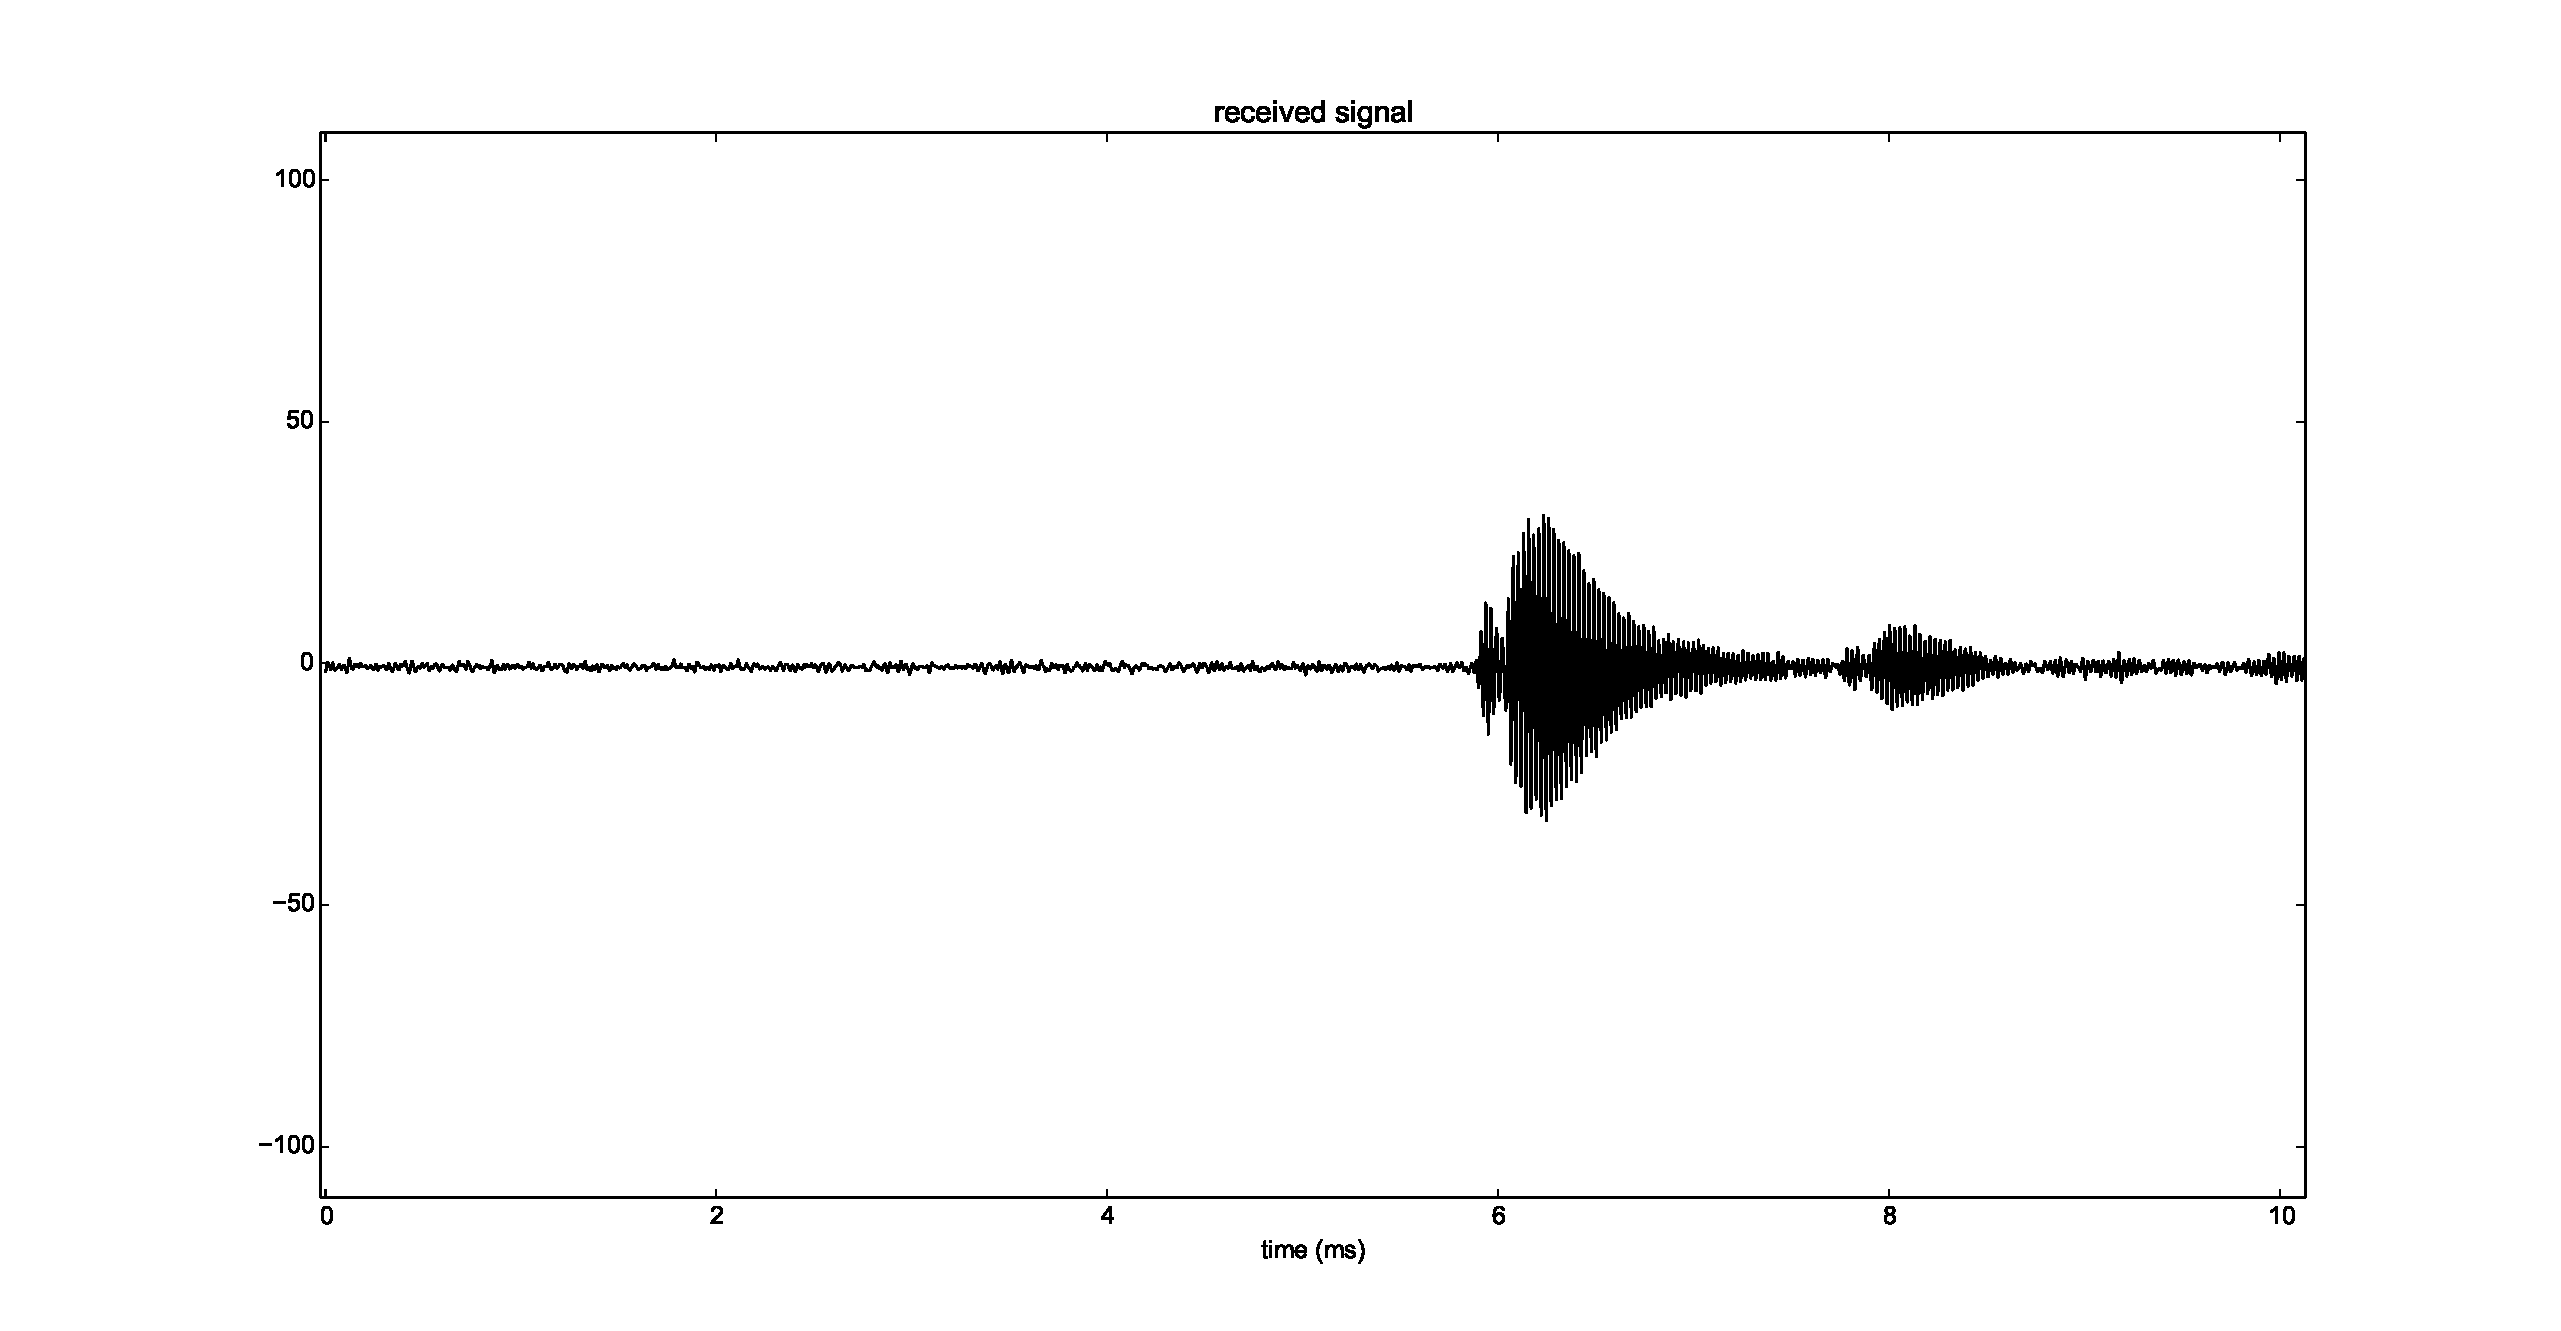
\includegraphics[width=1.15\textwidth, trim= 47mm 0mm 0mm 0mm,clip]{com_output_2m_1}
    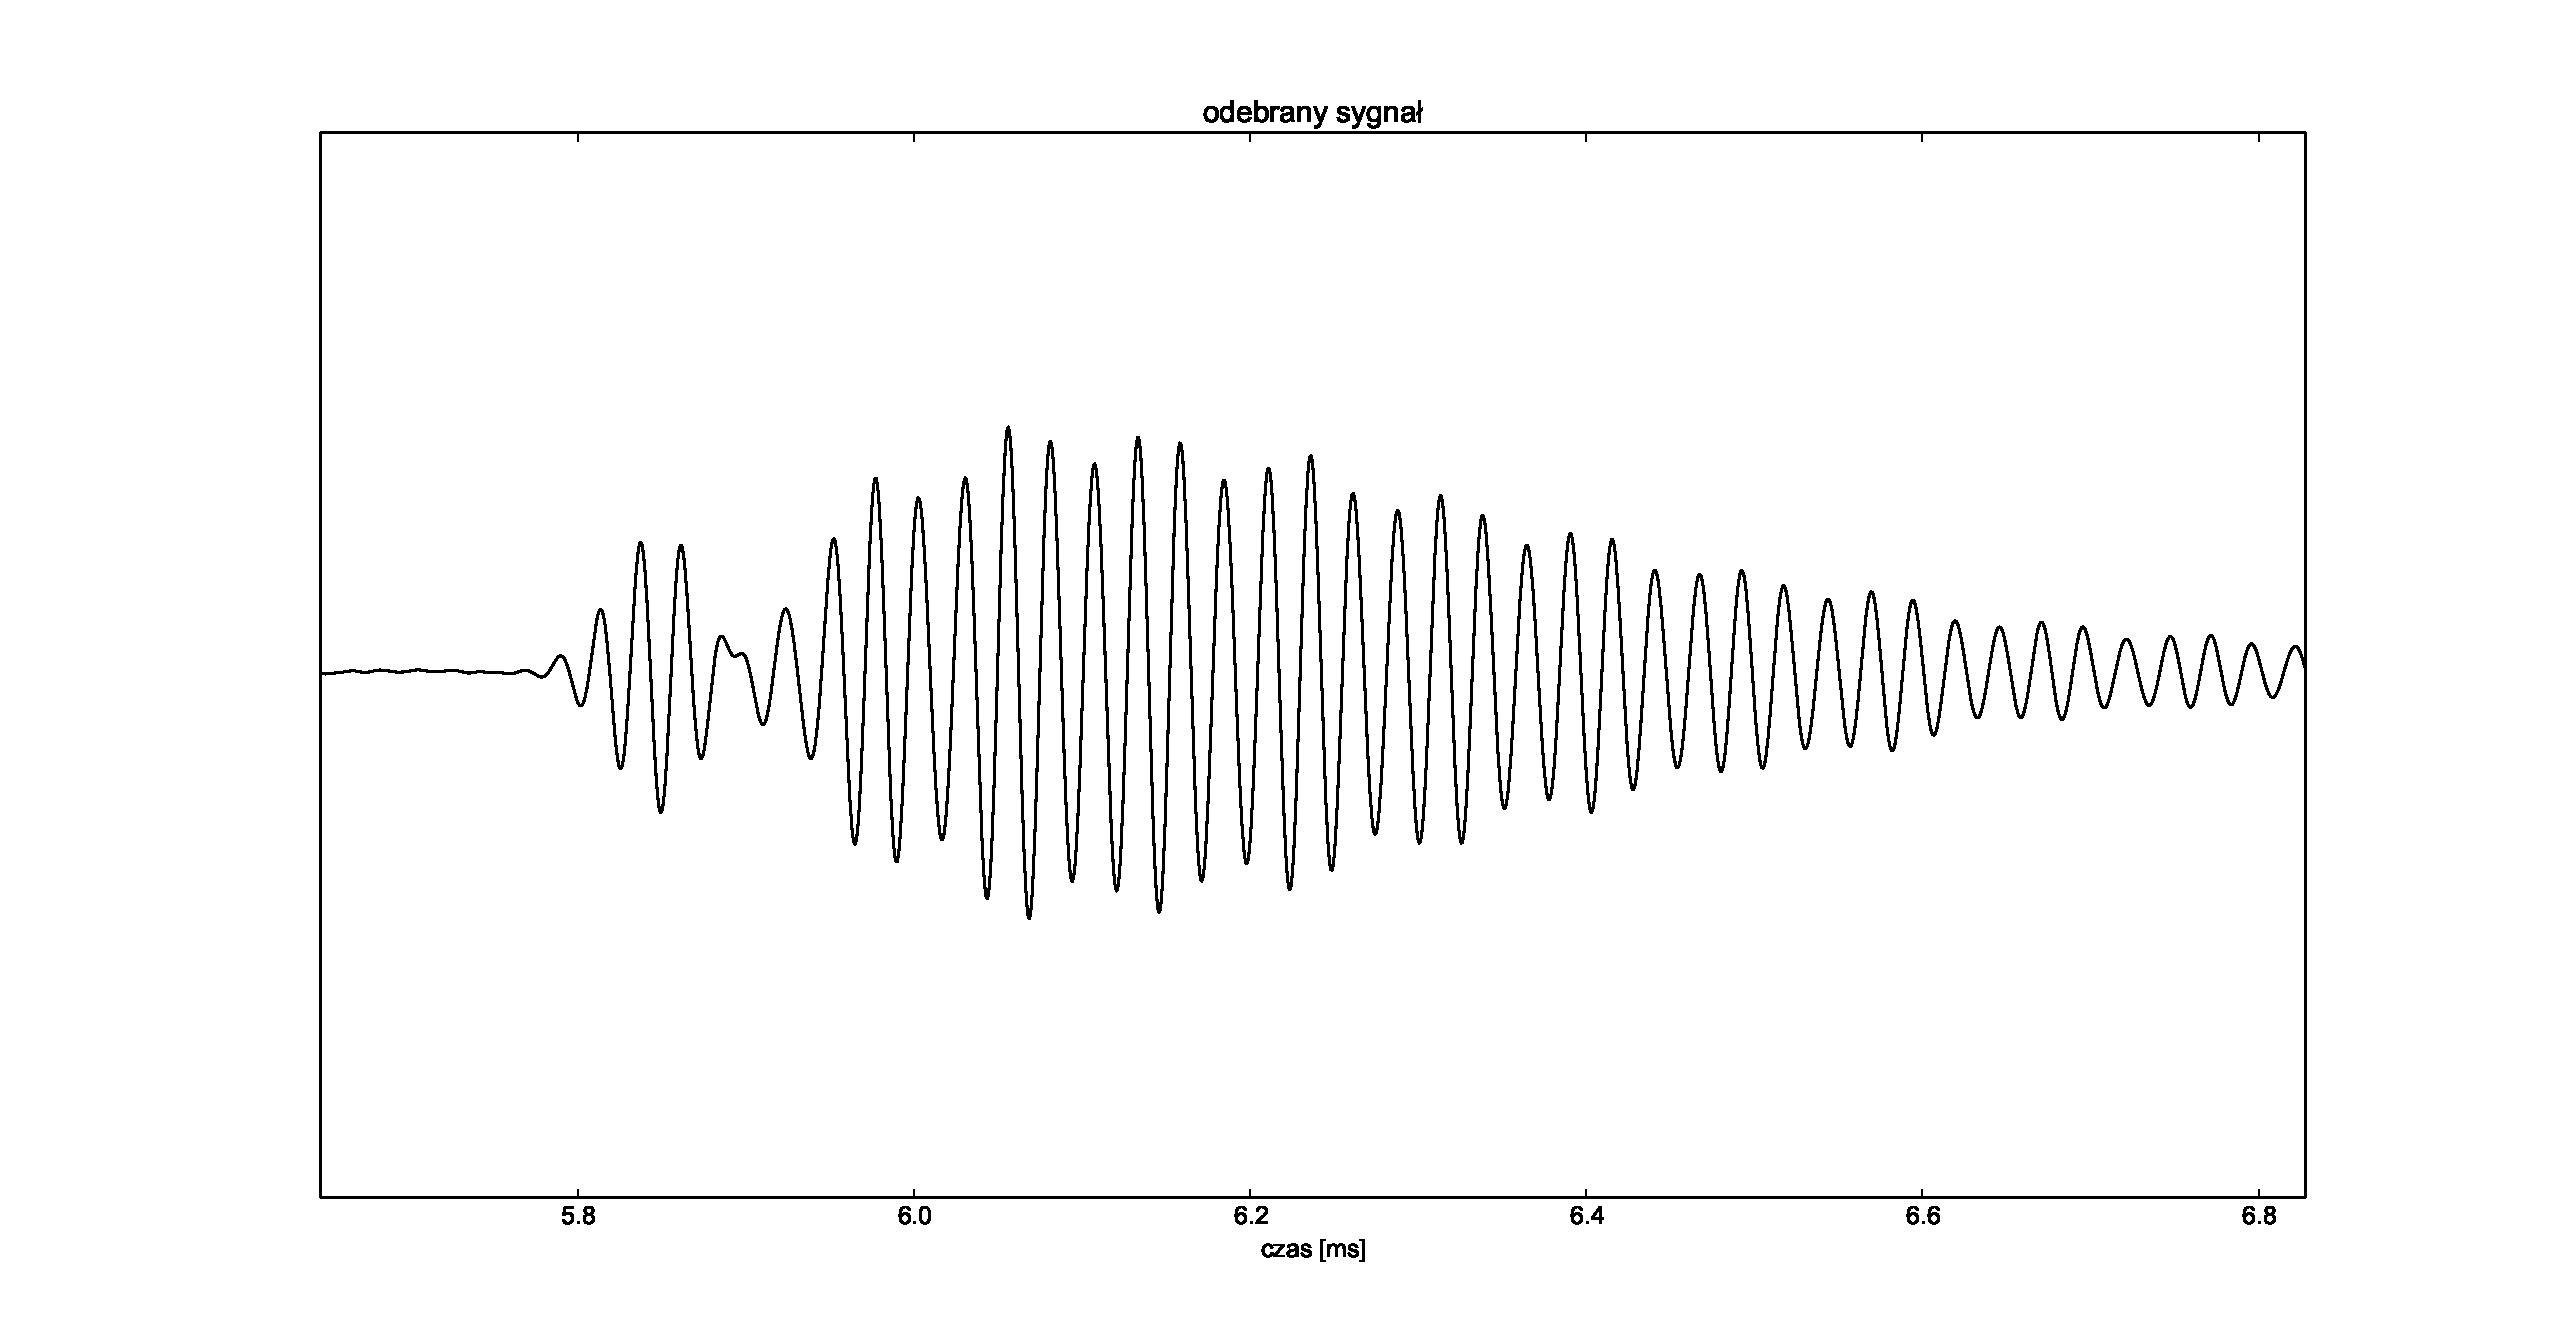
\includegraphics[width=1.15\textwidth, trim= 47mm 0mm 0mm 0mm,clip]{com_output_2m_2}
    \caption{sygnał odebrany przez moduł \textit{com.py}. 
    Odległość między nadajnikiem a odbiornikiem wynosi 2 metry.
    Na górnym wykresie po prawej stronie widoczny jest również sygnał odbity od podłogi.
    }
    \label{fig:com_output_2m}
\end{figure}


\section{moduł \textit{find\_pattern.py}}

Głównym modułem biblioteki \textit{mp3d} jest moduł \textit{find\_pattern.py}.
Odpowiada on za znalezienie \textit{wzorca} w odebranym sygnale z odbiorników,
